% +--------------------------------------------------------------------+
% | Sample Chapter 4
% +--------------------------------------------------------------------+

\cleardoublepage

% +--------------------------------------------------------------------+
% | Replace "This is Chapter 4" below with the title of your chapter.
% | LaTeX will automatically number the chapters.
% +--------------------------------------------------------------------+

\chapter{Implementación}
\label{makereference4}
A continuación, comenzaremos a exponer cómo hemos implementado nuestra aplicación, desde la arquitectura que hemos seguido, las tecnologías usadas para la parte 
frontend y la parte backend junto a las dificultades que nos hemos encontrado mientras trabajábamos y finalmente hablaremos de las herramientas de trabajo
utilizadas para facilitarnos el trabajo en equipo.
\section{Prototipos}
\label{makereference4.1}

\subsection{ARCore} 
\label{makereference3.6.1} 
\begin{flushleft}
    Al comenzar la fase de desarrollo de proyectos, pensamos que una de las tecnologías que debíamos 
    investigar y probar debía ser \textbf{ARCore}. Esto se debía a que, la empresa detrás de esta 
    tecnología es \textbf{Google} y esto podría significar que tendríamos más material de consulta 
    y ejemplos en comparación con otras tecnologías de fabricantes con menos recursos.
    \textbf{ARCore} se encuentra disponible para \textbf{Java}, \textbf{Unity}, \textbf{Unreal} e \textbf{iOS}. Comenzamos realizando el 
    "Quickstart" para \textbf{Android} y posteriormente para \textbf{Unity}. 
    Tras realizar los proyectos propuestos por \textbf{ARCore}, realizamos algún proyecto propio 
    para comprobar si la herramienta se ajustaba a la idea que teníamos para nuestro futuro proyecto.
    Tras realizar ambos proyectos, concluimos que, aunque \textbf{ARCore} reúne las características 
    necesarias para en un futuro convertirse en una de las tecnologías más importantes en Realidad Aumentada, 
    no íbamos a seleccionarla para nuestro proyecto por las siguientes razones:
    \begin{enumerate}
        \item \textbf{ARCore} dispone de mucha documentación para comenzar a usar la herramienta, pero poca para realizar tareas más complejas
        \item \textbf{ARCore} resulta muy útil para realizar superposiciones de modelos 3D sobre superficies, sin embargo, una de las funcionalidades más importantes que nuestra aplicación requería era la interacción con la realidad aumentada mediante el uso de botones, imágenes y la carga dinámica de elementos para posicionar en la pantalla de Realidad Aumentada e interaccionar con el usuario. En este sentido \textbf{ARCore} no está, por el momento, tan preparada como otras tecnologías.
    \end{enumerate}
    
\end{flushleft}
\subsection{Viro Media} 
\label{makereference3.6.2}
\begin{flushleft}
El objetivo del prototipo realizado con \textbf{Viro Media} es reconocer imágenes almacenadas en el dispositivo para mostrar texto y
 objetos virtuales. Además de probar tecnologías de desarrollo móvil web como en este caso \textbf{React Native}
 para plataformas \textbf{iOS} y \textbf{Android}.
\end{flushleft}
\begin{flushleft}
Comenzamos construyendo una interfaz sencilla con botones que nos redirigen a la escena de Realidad Aumentada.
Para esta interfaz utilizamos \textbf{NativeBase} que es una librería que nos permite
realizar una aplicación con apariencias de tipo \textbf{iOS} o \textbf{Android} según el dispositivo.
\end{flushleft}

\begin{figure}[htb]
    \centering
    \makebox[0pt][c]{%
    \begin{minipage}[b]{0.5\linewidth}
    \centering
      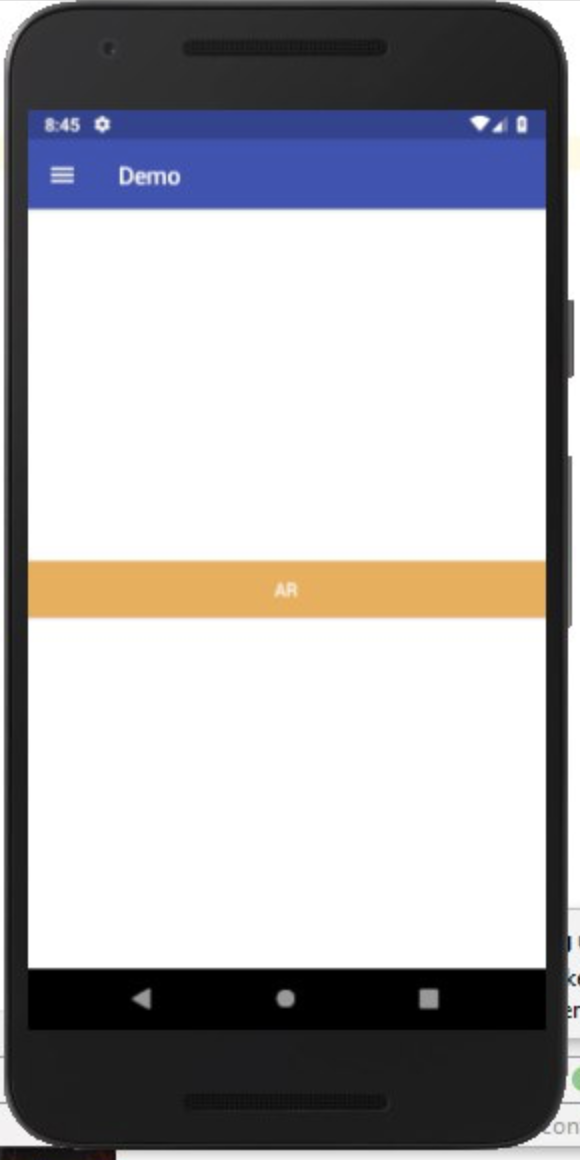
\includegraphics[scale=0.3]{figures/chapter-3/viromedia/android.png}
      \caption{Visualización con NativeBase en Android}
    \label{sva}
    \end{minipage}%
    \hspace{0.3cm}
    \begin{minipage}[b]{0.5\linewidth}
    \centering
     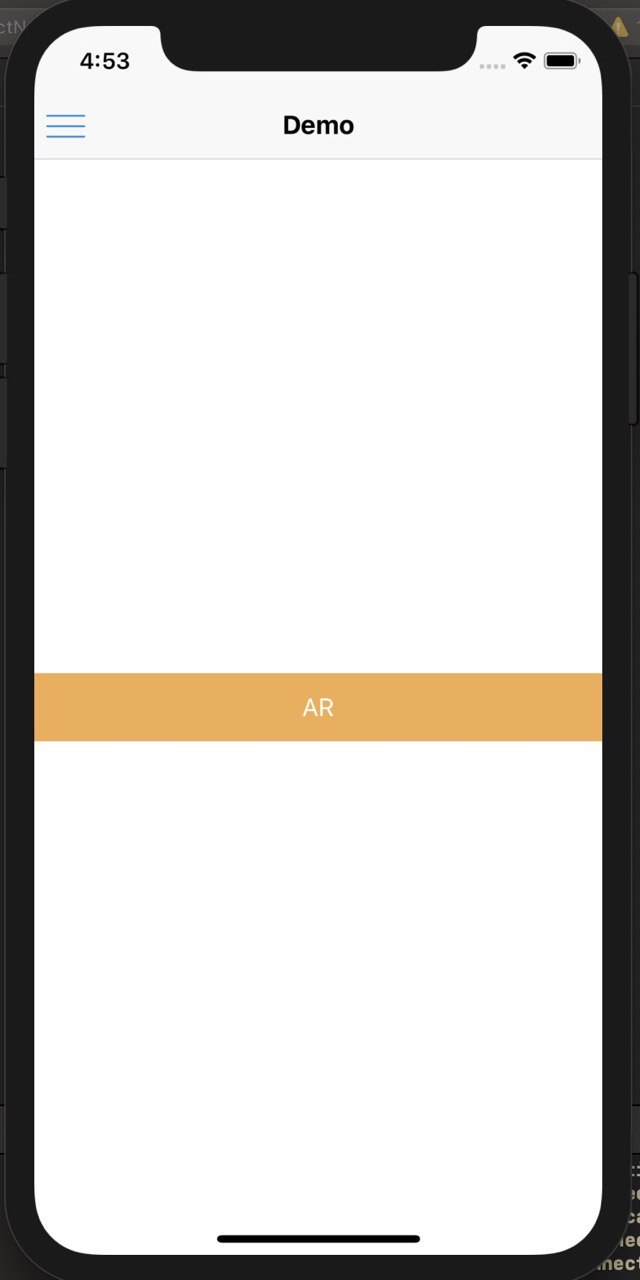
\includegraphics[scale=0.3]{figures/chapter-3/viromedia/ios.jpg}
      \caption{Visualización con NativeBase en iOS}
    \label{svb}
    \end{minipage}%
    }%
\end{figure}

\begin{flushleft}
Para la escena de Realidad Aumentada mostramos texto y al detectar el póster de Pantera Negra,
 reacciona mostrando una animación de dicho súper héroe saliendo del póster.
\end{flushleft}
 
\begin{figure}[H]
    \centering
    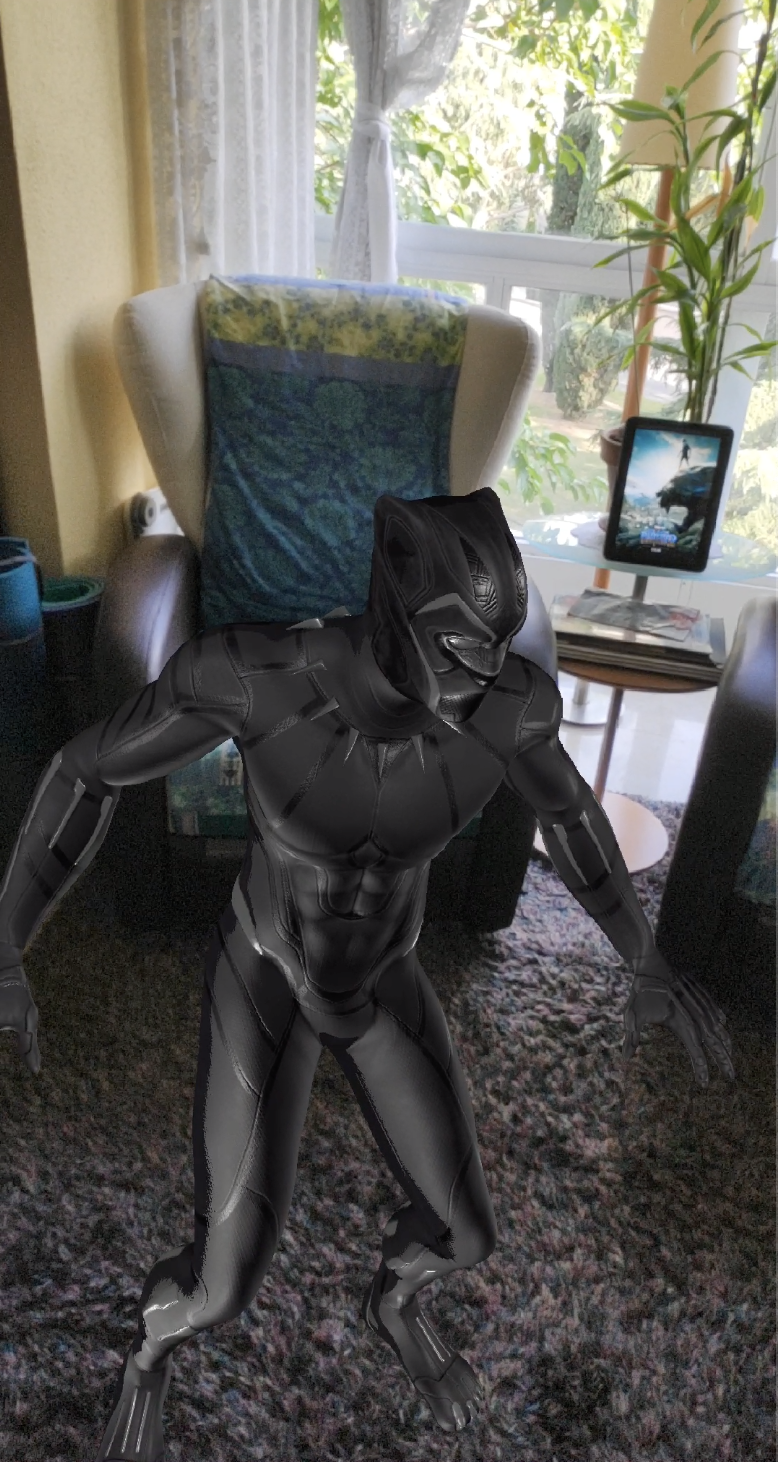
\includegraphics[width=3in]{figures/chapter-3/viromedia/blackpanther.png}
    \caption{Visualización de RA}
\end{figure}

\begin{flushleft}
Una de las ventajas que apreciamos fue la facilidad del lenguaje, en este caso \textbf{Javascript},
 utilizando la popular librería \textbf{ReactJS} y la buena documentación de \textbf{Viro Media}
 que hacían que el proceso de codificación fuera agradable.
\end{flushleft}
\begin{flushleft}
Uno de los problemas que presentaba este prototipo era que las dependencias de \textbf{Viro Media} entraban en conflicto con las de \textbf{NativeBase}
imposibilitándonos la forma de encontrar versiones compatibles. Utilizamos las últimas que, a pesar de lanzar
 advertencias, funcionaba en el ejemplo realizado.
Otro problema fue la compilación de la aplicación, \textbf{Viro Media} tiene una aplicación para probar lo
 que desarrollamos conectándose a nuestro ordenador a través de la red. El problema es
 que algunos recursos, como los iconos que utilizaba \textbf{NativeBase}, no eran descargados, por lo que la
 mejor forma era probar la versión compilada de \textbf{iOS} y \textbf{Android}. La forma de compilar
 la aplicación era un proceso costoso para los ordenadores, lento y con multitud de problemas según
 se ampliaban las librerías que se utilizan.
\end{flushleft}

\begin{flushleft}
La conclusión que obtuvimos de este prototipo fue que \textbf{Viro Media} y \textbf{React Native} son tecnologías muy prometedoras, pero debido a los
 problemas surgidos y a que todas sus versiones no eran estables vimos un claro riesgo para
 nuestro proyecto.
\end{flushleft}

\newpage
\subsection{Vuforia + Android} 
\label{makereference3.6.3} 
 
\begin{flushleft}
En este prototipo utilizamos la librería nativa de \textbf{Vuforia} para \textbf{Android} para 
realizar las pruebas de tecnología de reconocimiento de imágenes tanto en  
local como usando la nube que nos ofrecía \textbf{Vuforia}, para la posterior renderización
de objetos y textos.

Las características tecnológicas de este prototipo son las siguientes:
\end{flushleft}

\begin{enumerate}
    \item La librería de \textbf{Vuforia} para \textbf{Android} está diseñada a muy bajo nivel.
    \item \textbf{Vuforia} para dibujar en 3D usa la librería \textbf{OpenGL}.
    \item \textbf{OpenGL} utiliza una serie de espacios donde se van colocando los elementos: 
    \begin{enumerate}
        \item \textbf{Local space}: Es el espacio local de cada objeto.
        \item \textbf{World space}: Es el mundo donde se encuentran los objetos.
        \item \textbf{View space}: El mundo visto desde la perspectiva de la cámara.
        \item \textbf{Clip space}: Se integra con la pantalla del móvil y, definiendo los límites visibles, se establecen unas coordenadas de rango (-1,-1) - (1,1).
    \end{enumerate}
    \begin{flushleft}
        Las transformaciones de estos espacios se realizan mediante matrices 4x4, 
        en las que la primera fila hace referencia a la coordenada x, la segunda a la coordenada y y la 
        tercera a la coordenada z, mientras que la última columna hace referencia a los desplazamientos 
        de los objetos en esos 3 ejes.
        \end{flushleft}
        

        
            \begin{figure}[H]
                \centering
                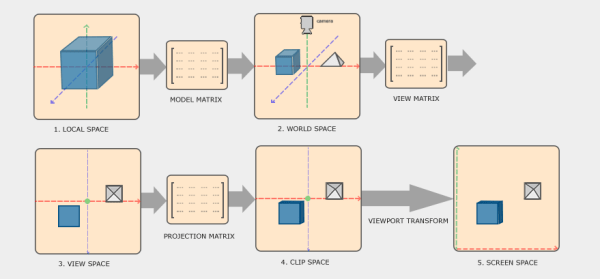
\includegraphics[width=5in]{figures/space-transformation.png}
                \caption{Esquema de los distintos espacios que usa OpenGL}
            \end{figure}

            \begin{figure}[H]
                \centering
                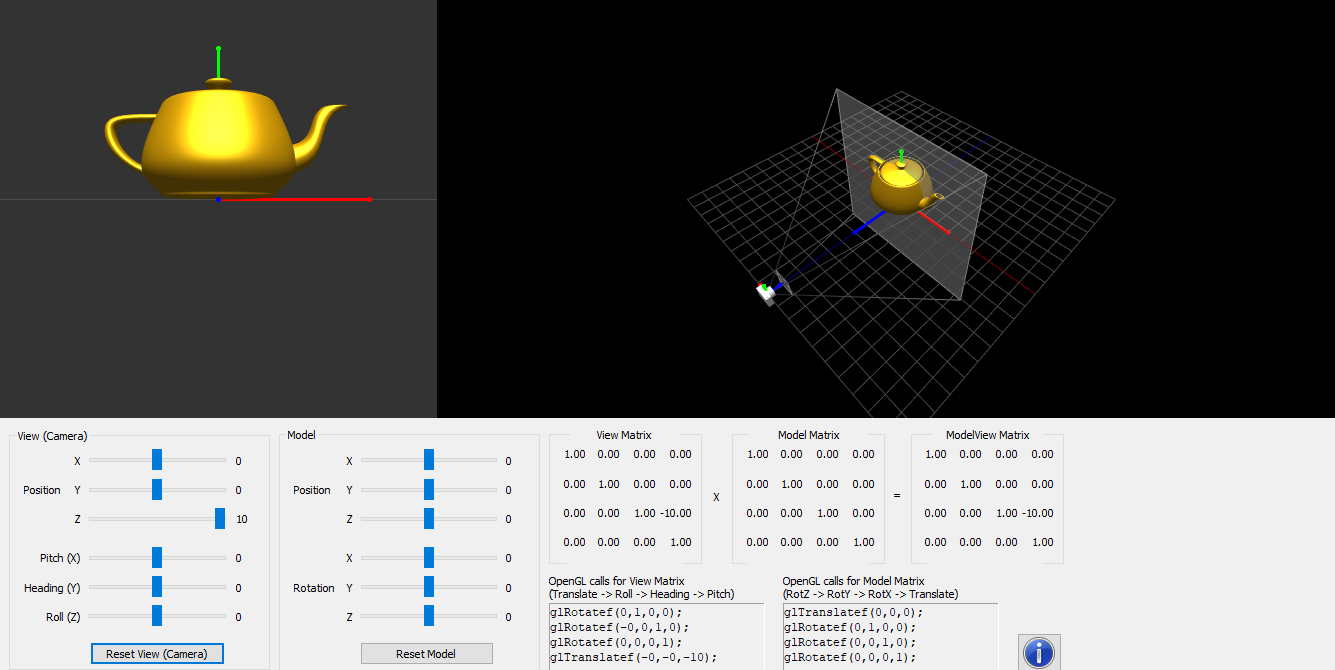
\includegraphics[width=5in]{figures/teapot.png}
                \caption{Ejemplo de un modelo en 3D}
            \end{figure}
    
    \item En \textbf{OpenGL} es necesario escribir código para que las tarjetas gráficas rendericen el modelo 3D,
    el lenguaje que se usa es \textbf{GLSL}. Este código de \textbf{GLSL} se escribe en forma de \textbf{String} y se llama a un método 
    que proporciona \textbf{OpenGL}.
    \begin{figure}[H]
        \centering
        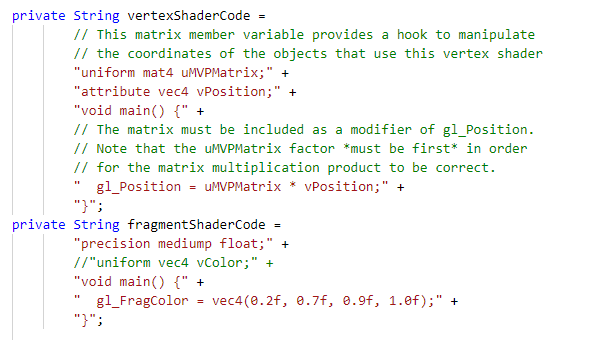
\includegraphics[width=5in]{figures/GLSL.png}
        \caption{Código en GLSL}
    \end{figure}
        
    \item Otro aspecto a tener en cuenta es que \textbf{OpenGL} solo nos ofrece lo básico, no nos ofrece métodos para dibujar 
    directamente objetos, sino que hay que seguir un pipeline de procesos para conseguir dibujar algo.
    \newline
    \begin{flushleft}
    Esto consiste en pasar un \textbf{array} de números (cada tres para definir un punto) 
    a las tarjetas gráficas, establecer triángulos entre los puntos (más arrays de números) 
    definir colores a partir de los puntos (más arrays)..., y con el código del shader, ejecutar 
    estos datos.
    \begin{figure}
        \centering
        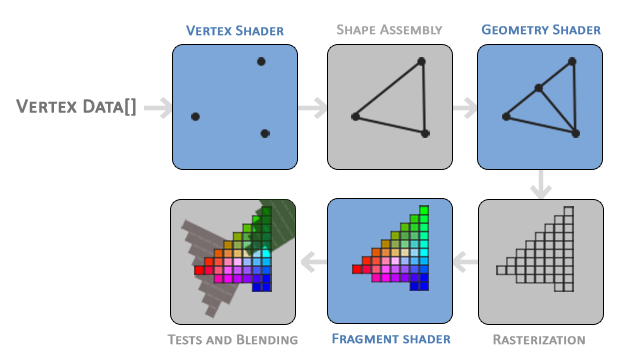
\includegraphics[width=4in]{figures/pipeline.png}
        \caption{Pipeline de la construcción de un modelo}
    \end{figure}
    \end{flushleft}
    \newpage
    \item Por último, como sólo ofrece métodos básicos, no hay métodos de escritura de texto, y la forma que 
    encontramos y que funcione fue usar un bitmap con los caracteres. Rechazamos esto por un principal motivo, para hacer que funciones hay que codificar a muy bajo nivel y 
    nos costaría mucho tiempo y esfuerzo.
    \begin{figure}
        \centering
        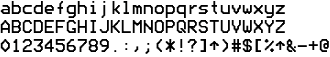
\includegraphics[width=5in]{figures/bitmap-font.png}
        \caption{Mapa de bits de caracteres usado}
    \end{figure}
\end{enumerate}
 

\newpage
\subsection{Vuforia + Unity} 
\label{makereference3.6.4}
\begin{flushleft}
    Para realizar este prototipo utilizamos \textbf{Unity} como herramienta básica para realizar la aplicación y \textbf{Vuforia} para dar soporte a la Realidad Aumentada.
    El prototipo a desarrollar consistió en un modelo 3D de un dragón que aparecía al detectar una imagen que previamente habíamos establecido como ``imagen objetivo''.
\end{flushleft}
    \begin{figure}[H]
        \centering
        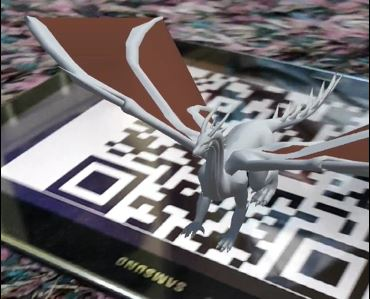
\includegraphics[width=5in]{figures/prototipoUnity.jpg}
        \caption{Modelo en 3D que aparecía al detectar la imagen}
    \end{figure}
\begin{flushleft}
    Pese a que nadie del equipo había utilizado \textbf{Unity} previamente el resultado fue bastante positivo ya que:
    \begin{enumerate}
    \item \textbf{Unity} resultó ser intuitivo y relativamente fácil en cuanto al aprendizaje de las funcionalidades básicas.
    \item \textbf{Vuforia} parecía estar muy probada e incluía de serie muchas funcionalidades.
    \item \textbf{Vuforia} tenía la opción de utilizar un \textbf{Cloud} para almacenar las imágenes objetivo.
    \end{enumerate}
\end{flushleft}

\subsection{Vuforia + Unity + Android} 
\label{makereference3.6.5}
\begin{flushleft}
Una vez realizado el prototipo en \textbf{Vuforia} con \textbf{Unity} comenzamos a investigar cómo realizar el resto de la aplicación que no requería de Realidad Aumentada.
\break
Hasta este momento teníamos claro que \textbf{Vuforia} con \textbf{Unity} era la mejor combinación para realizar la parte de Realidad Aumentada, sin embargo, \textbf{Unity} no era igual de intuitivo ni eficaz a la hora de realizar tareas propias de una aplicación "normal", como el desarrollo de interfaces o la lógica.
\break
Por este motivo intentamos buscar la opción de realizar una aplicación en la que la Realidad Aumentada estuviese diseñada en \textbf{Unity} con \textbf{Vuforia} y el resto de la aplicación en Android.
\end{flushleft}
\begin{figure}[H]
        \centering
        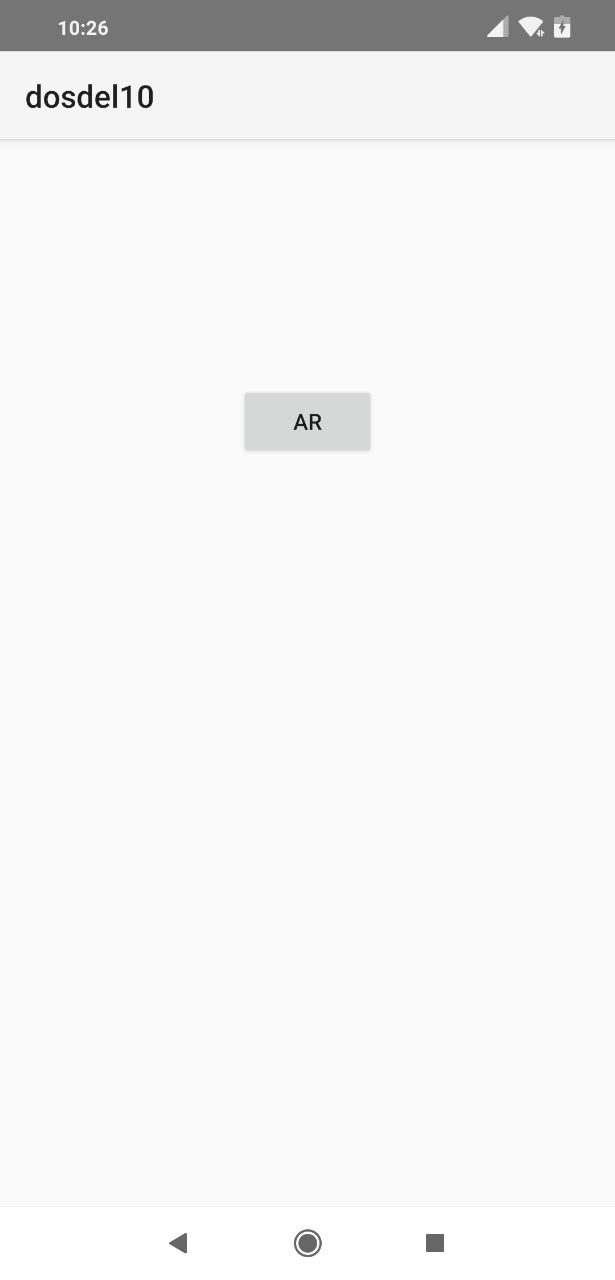
\includegraphics[width=1in]{figures/androidUnityVuforia.jpg}
        \caption{Botón que comunicaba Android con Unity}
\end{figure}
\begin{flushleft}
    Finalmente conseguimos tener ambos proyectos independientes, la Realidad Aumentada se desarrollaba en \textbf{Unity} con \textbf{Vuforia} y se exportaba a un proyecto Android donde se encontraba el resto de la aplicación.
    Esto nos permitía realizar la Realidad Aumentada con la herramienta que tras las primeras tomas de contacto habíamos comprobado que era la mejor (\textbf{Unity} con \textbf{Vuforia}) y del mismo modo realizar el resto de la aplicación con la mejor herramienta para esta parte (AndroidStudio).
\end{flushleft}
\begin{flushleft}
    Tras realizar este prototipo, consideramos que estas herramientas podrían ser las que usásemos en la aplicación final puesto que:
    \begin{enumerate}
    \item Como ya habíamos descubierto en el prototipo anterior, \textbf{Unity} era una herramienta muy completa y junto con \textbf{Vuforia} nos proporcionaban todas las herramientas necesarias para cumplir con los casos de uso de Realidad Aumentada que teníamos en mente.
    \item Al haber encontrado la forma de combinar \textbf{Unity + Android} no teníamos que renunciar a ninguna de las dos herramientas. Lo que nos permitía explotar las cosas buenas de ambas herramientas.
    \item La comunicación entre \textbf{Unity} y Android era relativamente sencilla pese a ser dos proyectos distintos.
    \end{enumerate}
\end{flushleft}

\newpage
\subsection{Server en Spring} 
\label{makereference3.6.6}

\begin{flushleft}
    Para la realización de la parte backend de la aplicación decidimos
    incorporar la tecnología de \textbf{Spring} para codificar un \textbf{servicio web REST} en \textbf{Java}
    y el acceso a datos mediante \textbf{MySQL}.
\break
\break
    Para el prototipo seguimos el siguiente tutorial: 
\newline
Cómo crear un microservicio o servicio web REST con Spring Boot\cite{tutorialspring}
\break
    que consistía en 3 partes bien definidas para la creación de dicho \textbf{servicio web REST} para la gestión de una entidad de contactos muy simple, se puede observar su estructura
    en la figura 3.6.
    \begin{figure}[H]
        \centering
        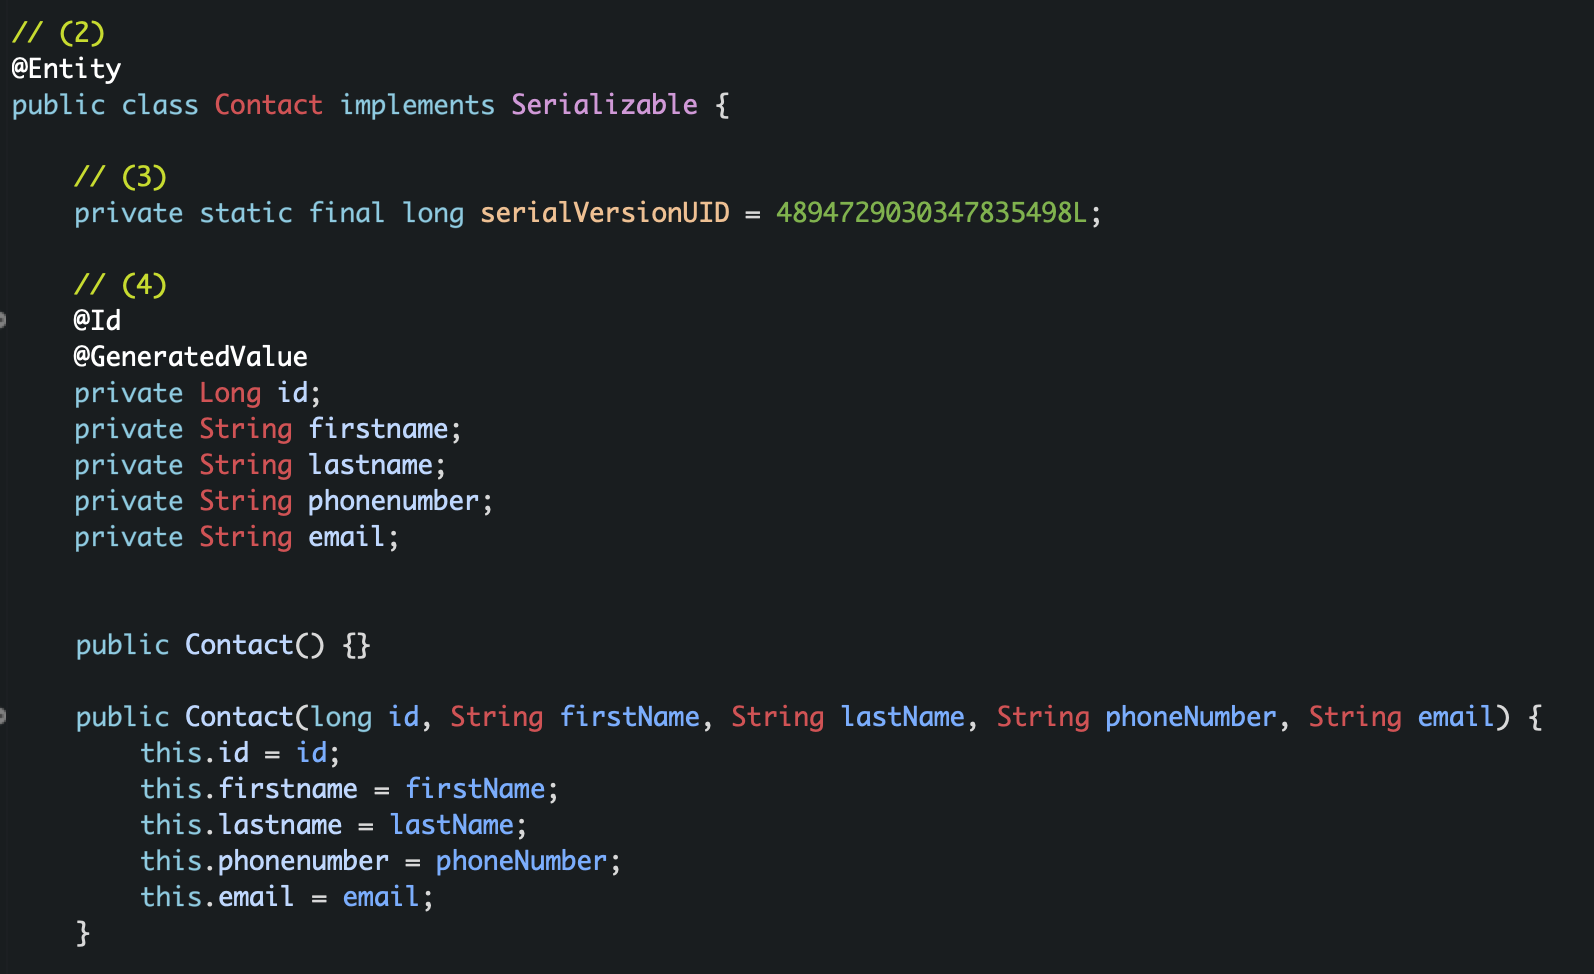
\includegraphics[width=6in]{figures/ContactsEntity.png}
        \caption{Entidad de Contactos}
    \end{figure}
\break
\break
    También se investigaron distintas formas de realizar el acceso a la base de datos desde el servidor, pero finalmente nos decantamos por usar la
    clase \textbf{JPARepository} o \textbf{CRUDRepository}, las cuales nos ofrecen ya implementados los métodos típicos de las operaciones \textbf{CRUD}, además de la opción 
    de poder crear nuestros propios métodos.
\end{flushleft}

\begin{flushleft}
    Para poder probar las distintas peticiones de tipo \textbf{POST} y \textbf{GET}, que realizamos en local, usamos la herramienta 
    \textbf{Postman}, ver figura 3.7.
    \begin{figure}[H]
        \centering
        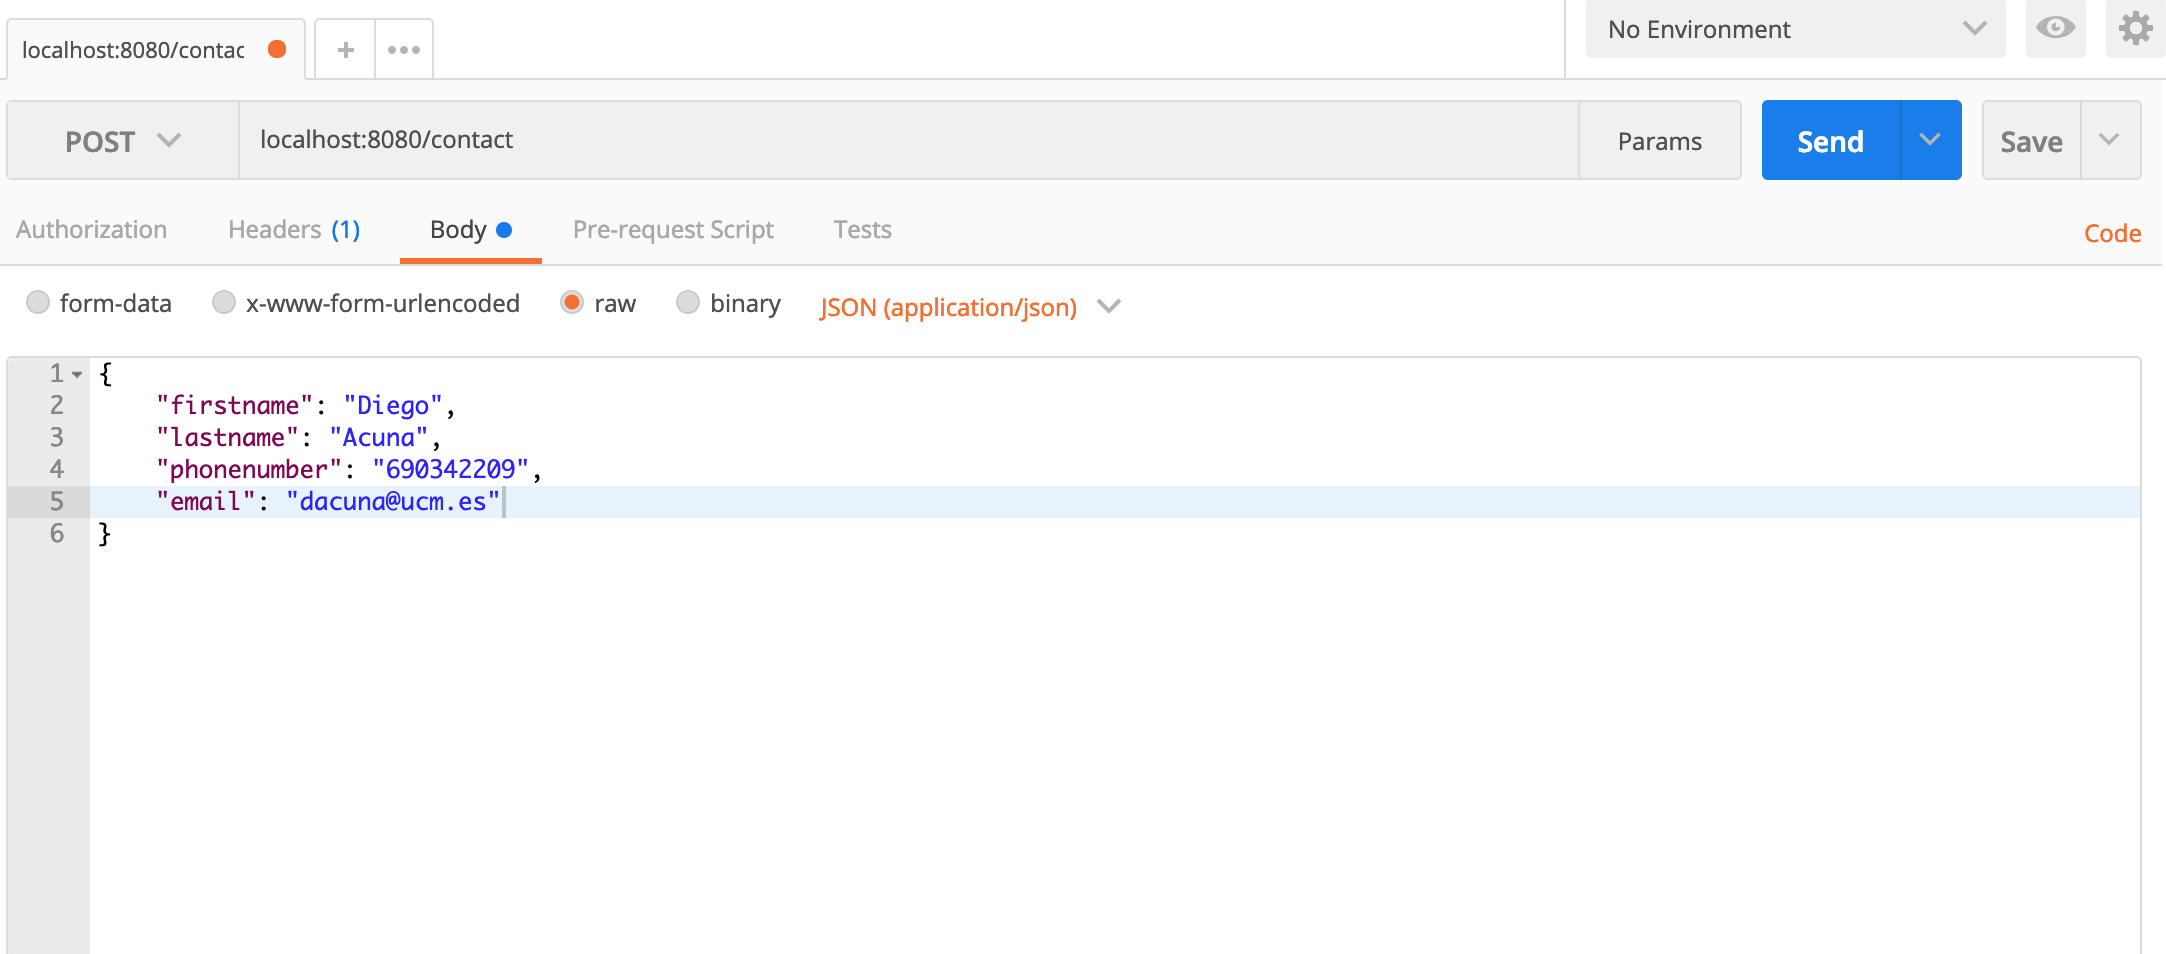
\includegraphics[width=6in]{figures/Postman.png}
        \caption{Postman}
    \end{figure}
    Para este prototipo decidimos usar \textbf{MySQL} como sistema de gestión de bases de datos relacional, aunque
    a la hora de probar a levantar nuestro servidor de prueba tuvimos que rehacer este prototipo, además de adaptarlo para 
    que gestionara entidades de películas, y que usara \textbf{PostgreSQL}, además de cambiar una serie de anotaciones y limpiar 
    el archivo \textbf{pom.xml} de líneas de código innecesarias, ver figura 3.8, que es el que contiene las dependencias de nuestro proyecto.
    \begin{figure}[H]
        \centering
        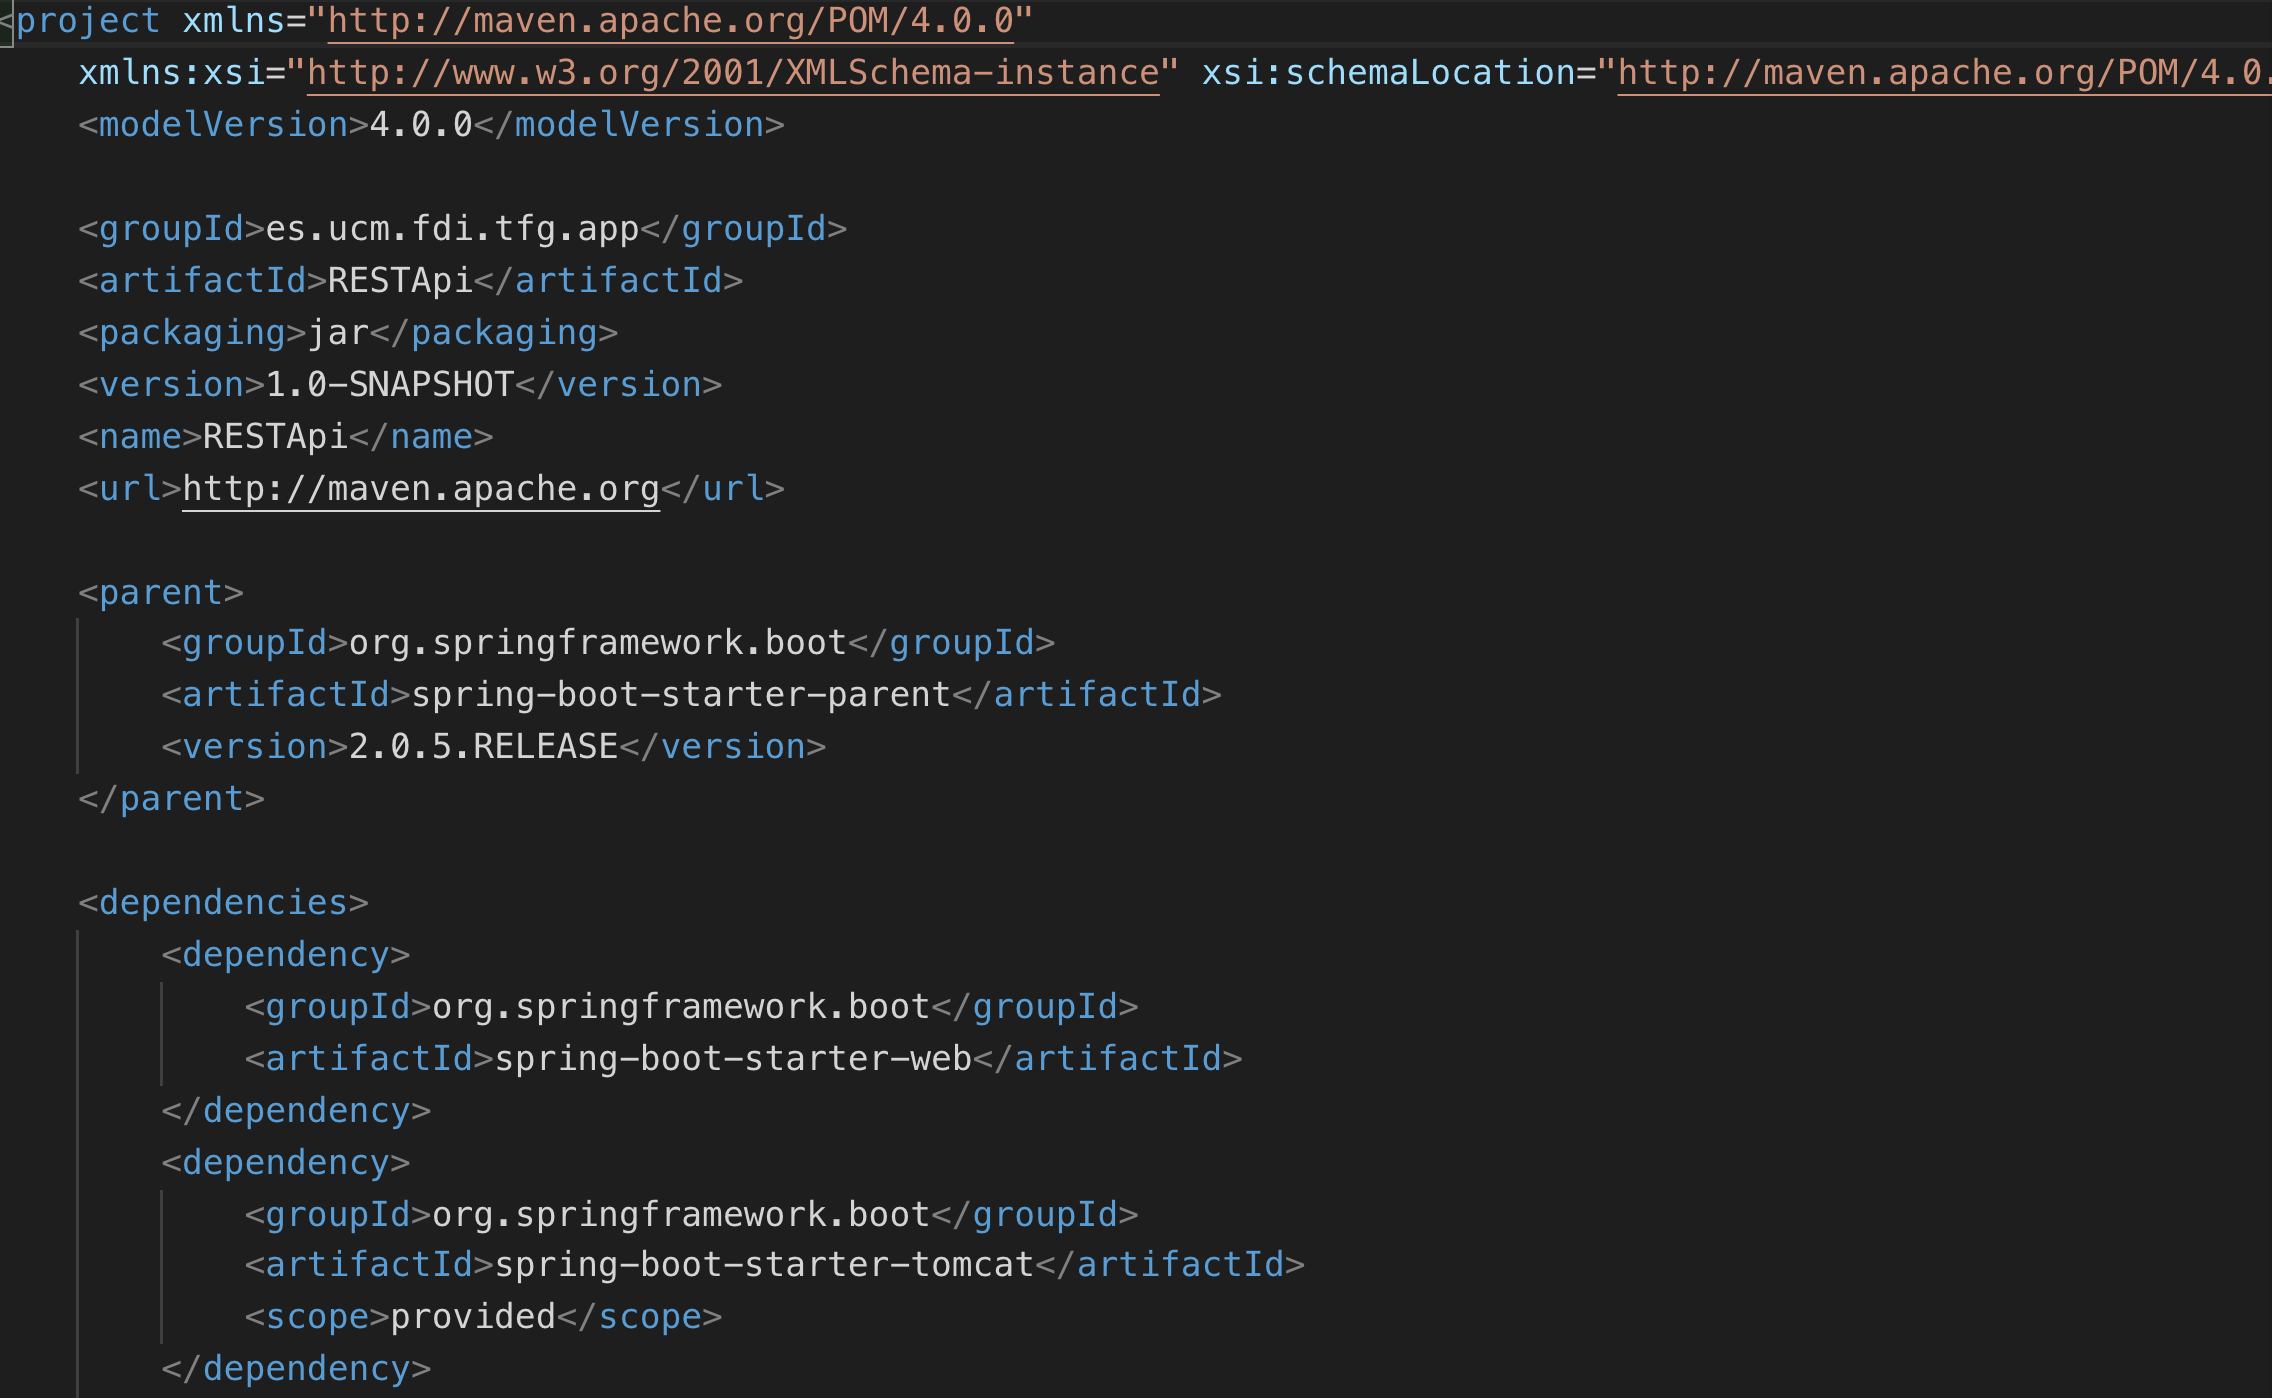
\includegraphics[width=6in]{figures/PomXML.png}
        \caption{Archivo pom.xml}
    \end{figure}
\end{flushleft}
\section{Arquitectura}
\label{makereference4.1}
En cuanto a la arquitectura usada en nuestra aplicación hemos adjuntado un esquema que podemos observar en la figura 4.1. Nuestro cliente estará implementado tanto en \textbf{Android}
como en \textbf{Unity}, la aplicación general está en \textbf{Android}, mientras que la parte de realidad aumentada está desarrollada en \textbf{Unity} y usa \textbf{Vuforia}. Para el reconocimiento
de imágenes con \textbf{Vuforia} usamos un \textbf{Cloud} gratuito que nos ofrece para almacenar las imágenes ya que, tener todas las imágenes en la misma aplicación la cargaría de un peso innecesario.
Para la parte del servidor, hemos realizado una \textbf{API Rest} con \textbf{Spring}, usando además una base de datos relacional en \textbf{PostgreSQL}. 
\begin{figure}[H]
    \centering
    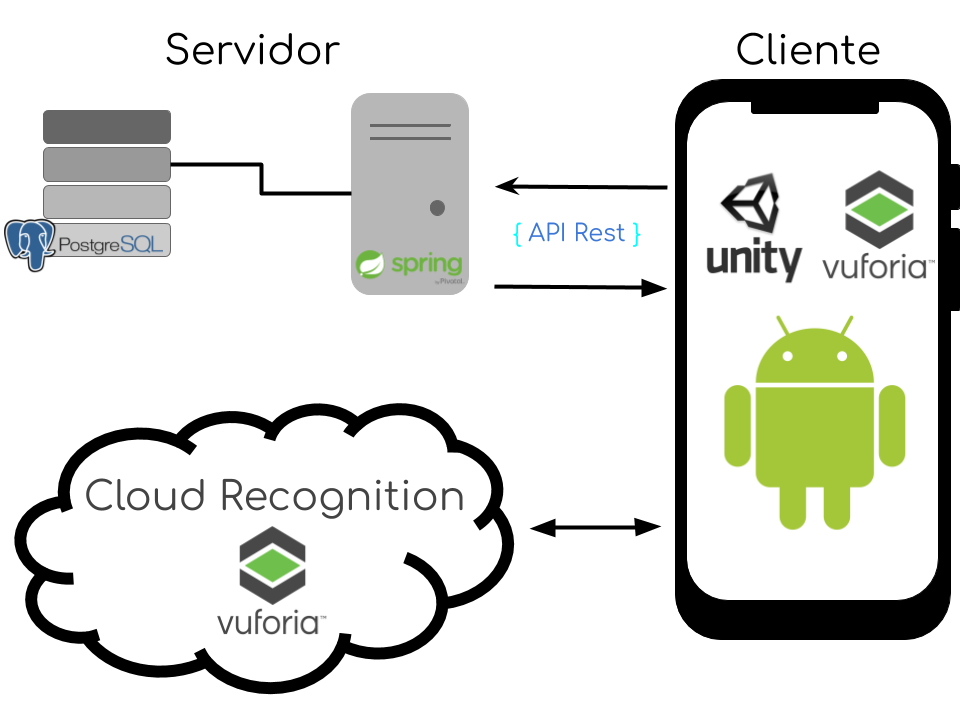
\includegraphics[width=6in]{figures/chapter-4/arquitectura.png}
    \caption{Arquitectura}
\end{figure}
\section{Servidor}
\label{makereference4.2}
Nuestro servidor está programado en \textbf{Java}, usando el framework \textbf{Spring} para la creación de una \textbf{API Rest} que mediante peticiones \textbf{HTTP} y una base de datos relacional en \textbf{PostgreSQL} nos proporcionará
toda la información necesaria para alimentar de datos a nuestro cliente. El servidor necesita ser desplegado para que la aplicación pueda tener un uso real por lo que conseguimos desplegarlo de forma gratuita en \textbf{Heroku}, que además ofrece
facilidades para desplegar un servidor creado mediante \textbf{Spring}, por lo que nos facilitó el trabajo considerablemente. También se encuentra en el servidor la implementación del sistema de recomendación.
\subsection{Despliegue en Heroku}. 
\label{makereference4.2.1}
Para el despliegue de la aplicación de servidor utilizamos Heroku. Esta plataforma nos ofrece un alojamiento gratuito con las características suficientes para el desarrollo del proyecto.
\begin{figure}[H]
    \centering
    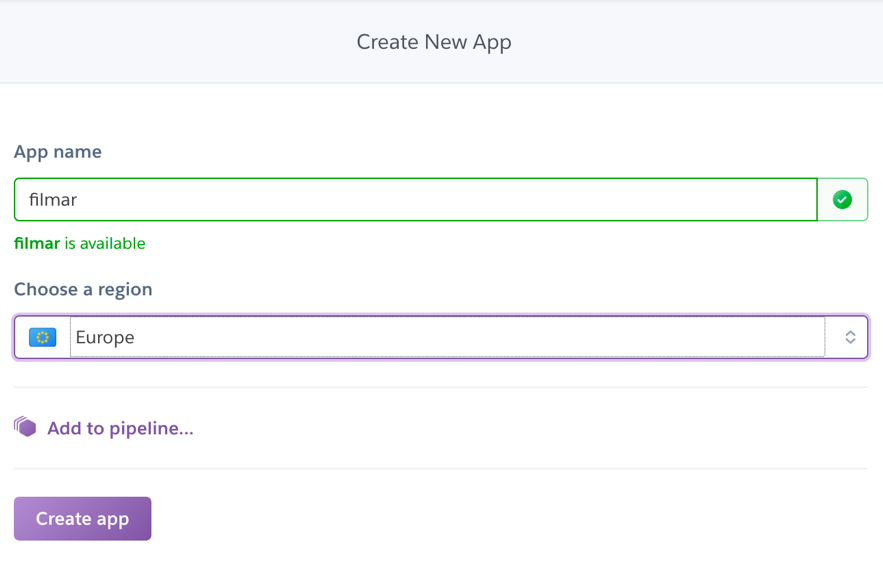
\includegraphics[width=6in]{figures/chapter-4/heroku_1.png}
    \caption{Crear nueva aplicación en Heroku}
\end{figure}
Una vez tenemos una cuenta en la plataforma creamos una nueva aplicación a la cual daremos un nombre como vemos en la figura 4.2 y este nombre a su vez será parte de la URL pública.
\begin{figure}[H]
    \centering
    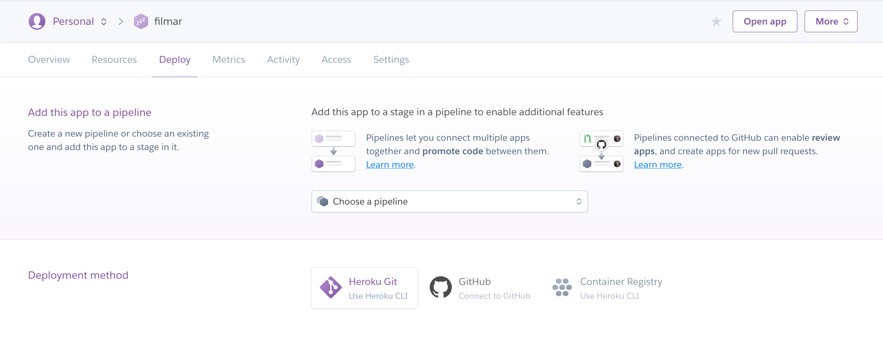
\includegraphics[width=6in]{figures/chapter-4/heroku_2.png}
    \caption{Configuración de la aplicación}
\end{figure}
Cuando creemos la aplicación accederemos a la configuración en la que veremos opciones como en la figura 4.3.
\begin{figure}[H]
    \centering
    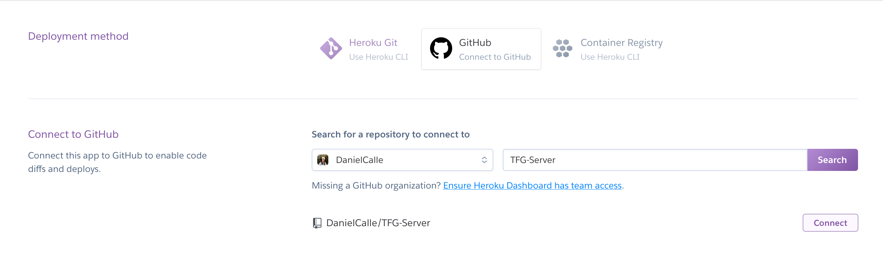
\includegraphics[width=6in]{figures/chapter-4/heroku_3.png}
    \caption{Métodos de despliegue}
\end{figure}
En la figura 4.4 vemos que nos ofrece diversos métodos de despliegue:
\begin{itemize}
    \item Heroku Git
    \item GitHub
    \item Container Registry
\end{itemize}
Elegimos la opción de GitHub que nos proporciona un despliegue fácil y rápido. Tenemos que vincular la cuenta de nuestro GitHub (Importante ser el dueño del repositorio).
\begin{figure}[H]
    \centering
    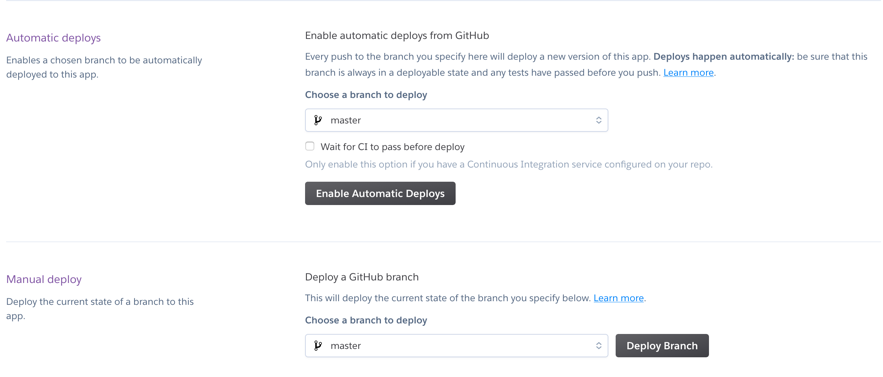
\includegraphics[width=6in]{figures/chapter-4/heroku_4.png}
    \caption{Opciones de despliegue utilizando Github}
\end{figure}
Una vez vinculada la cuenta de GitHub tenemos dos métodos de despliegue como vemos en la figura 4.5. Un método automático para desplegar los cambios de una rama del repositorio que se accionara cada vez que subamos cambios y otro método manual que se desplegará sólo cuando presionemos el botón. 
Cuando elijamos una de las opciones, la aplicación estará lista para usarse.
\section{Aplicación}
\label{makereference4.3}
Nuestra aplicación está implementada principalmente en \textbf{Android}, las interfaces principales para el uso de los planes, recomendaciones y acceso a la información de las películas guardadas han sido desarrolladas mediante \textbf{Android Studio}. Sin embargo,
la parte del cliente que otorga el gran valor a nuestra aplicación está desarrollada en \textbf{Unity} y el uso de \textbf{Vuforia}, todas las escenas que aparecen al reconocer carteles de películas e imágenes de usuarios fueron implementadas de esta forma. \textbf{Vuforia} además nos ofrece un
servicio de \textbf{Cloud} para el almacenamiento de imágenes, a las cuales les asocia una valoración según lo fácil que le resultará a la aplicación reconocerla y un identificador único (\textbf{UUID}), que es el que usaremos para guardar la distinta información de dicha película o usuario en la base de datos.
La parte de la aplicación realizada en \textbf{Unity}, utiliza una serie de clases de la parte desarrollada en \textbf{Android} para realizar las peticiones al servidor y así poder mostrar información específica cuando se reconoce una cierta imagen.
Al principio hicimos que las dos partes realizaran las peticiones en sus respectivos lenguajes, pero decidimos que sería mejor que el acceso a la capa de datos se realizara por el mismo sitio y así conseguir que las distintas capas estuvieran separadas.
Además, en un principio, las imágenes que mostramos en la parte de \textbf{Android} se almacenan en \textbf{Google Drive} y mediante la librería de \textbf{Picasso} las obtenemos en tiempo de ejecución, esto se ha implementado de esta forma por la misma razón por la que tenemos las imágenes a reconocer en un \textbf{Cloud}.
Finalmente, debido al coste en tiempo de esta operación y tras debatirlo con nuestros directores del Trabajo de Fin de Grado, hemos decidido guardar dichas imágenes en el mismo servidor para su rápida obtención.


Como la mayor parte de la aplicación está implementada en \textbf{Android Studio}, la estructura de ésta se adapta a lo que ofrece el \textbf{IDE}, consistiendo en el flujo de unas actividades y fragmentos que explicaremos a continuación.

\begin{figure}[H]
    \centering
    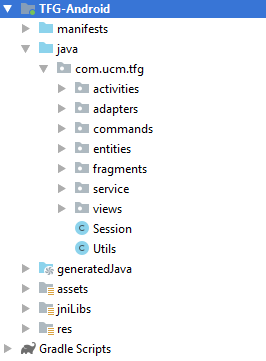
\includegraphics[width=3in]{figures/chapter-4/android_project_structure.png}
    \caption{Estructura de ficheros del proyecto android}
\end{figure}

\subsection{Actividades}
\label{makereference4.3.1}
Son los componentes de la aplicación que representan una pantalla con la que los usuarios pueden interactuar para realizar una determinada acción.

\begin{figure}[H]
    \centering
    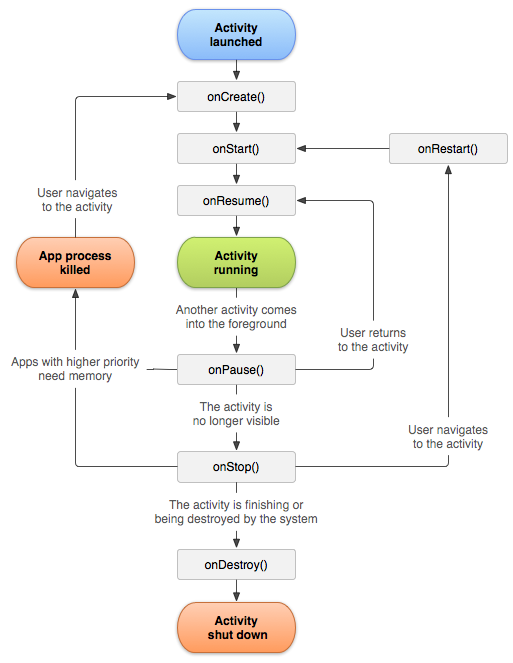
\includegraphics[width=3in]{figures/chapter-4/activity_lifecycle.png}
    \caption{Ciclo de vida de una actividad}
\end{figure}

Entre nuestras actividades podemos destacar dos: 
\begin{itemize}
    \item \textbf{MainActivity:} La primera actividad (actividad principal) que se activa al iniciar la aplicación, la cual comprueba el estado de sesión del usuario, si está logueado se queda en la actividad, y si no, se redirige al usuario a otra actividad (LoginActivity) para que pueda iniciar sesión o registrarse. En MainActivity se encuentra un paginador (ViewPager) de 3 fragmentos, donde cada fragmento representa las interfaces de planes, recomendaciones y películas guardadas correspondientemente.
    \item \textbf{UnityPlayerActivity:} Se trata de una actividad especial que nos permite comunicar la parte desarrollada en \textbf{Unity} con nuestro proyecto \textbf{Android}. Aquí se encuentran llamadas a funciones desde la parte de Unity, se realizan las órdenes y se devuelven a Unity.
\end{itemize} 

\subsection{Adaptadores}
\label{makereference4.3.2} 
Son elementos de manipulación de datos que se aplican a vistas y componentes. En el proyecto se les ha dado mucho uso a las vistas de tipo \textbf{RecyclerView} para representar listas de objetos. Para manejar los datos de cada elemento de la lista, se ha utilizado un \textbf{RecyclerView.Adapter}, el cual manipula cada dato correspondiente a un elemento de la lista. También se han creado otros adaptadores, como uno para manejar tres fragmentos dentro de una actividad, como hemos dicho anteriormente al describir la actividad principal (MainActivity).

\subsection{Comandos}
\label{makereference4.3.3}
Aquí se encuentran todos los elementos relacionados con el patrón comando y ha sido diseñado para realizar la conexión con la parte del proyecto desarrollado en Unity.

\begin{figure}[H]
    \centering
    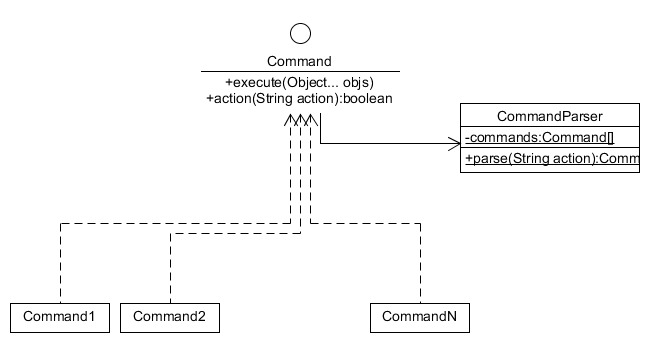
\includegraphics[width=3in]{figures/chapter-4/command_pattern.png}
    \caption{Patrón comando}
\end{figure}

Este patrón permite solicitar una operación a un objeto sin conocer realmente el contenido de esta operación, ni el receptor real de la misma. Para ello se encapsula la petición como un objeto, lo que además facilita la parametrización de los métodos.

La implementación de este patrón consiste en crear una interfaz en la cual las demás clases (comandos) la implementan. La interfaz tiene dos funciones: 
\begin{itemize}
    \item  \textbf{execute} para ejecutar la tarea.
    \item  \textbf{action} para comprobar si este comando es el indicado para ejecutar la tarea. 
\end{itemize} 
Por otro lado, tenemos una clase llamada \textbf{CommandParser}, encargada de buscar el comando apropiado para su ejecución.

\subsection{Entidades}
\label{makereference4.3.4}
Todos los modelos de datos que podemos recibir del servidor como planes, películas, usuarios, etc. Son representados por entidades en nuestro proyecto de \textbf{Android}, con los mismos atributos que tienen sus entidades correspondientes en el servidor.

\subsection{Fragmentos}
\label{makereference4.3.5}
Representan un comportamiento o una parte de la interfaz de usuario en una actividad.

\begin{figure}[H]
    \centering
    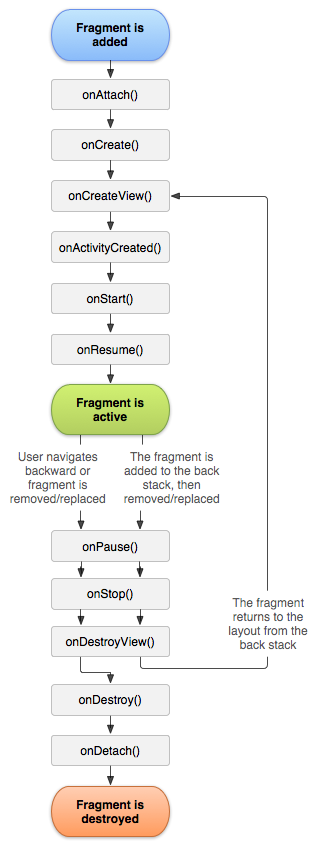
\includegraphics[width=3in]{figures/chapter-4/fragment_lifecycle.png}
    \caption{Ciclo de vida de un fragmento}
\end{figure}

Se utilizan para formar una vista compuesta de paginación en una actividad. 

\subsection{Servicios}
\label{makereference4.3.6}
Se trata de un conjunto de clases que solo poseen métodos estáticos para llevar a cabo peticiones \textbf{HTTP} al servidor. Se ha creado una clase genérica para la creación y llamada de peticiones \textbf{HTTP}, se ha diseñado de manera que las respuestas se devuelvan en forma de \textbf{callback} para un uso más sencillo.

\subsection{Vistas}
\label{makereference4.3.7}
Entre los componentes que ofrece \textbf{Android} hay algunas funcionalidades que no soporta. Por ello hemos creado componentes personalizados para satisfacer a estas funcionalidades:
\begin{itemize}
    \item \textbf{AnchorVisibilityBehavior:} Implementa un comportamiento que aplicado a una vista determinada, genera el comportamiento deseado. En este caso el comportamiento es la visibilidad que tiene algunas vistas colocadas en un toolbar (depende de su altura). 
    \item \textbf{CustomViewPager:} ViewPager es lo que se usa en el MainActivity para colocar los tres fragmentos. Se crea esta clase para desactivar la acción de poder pasar los fragmentos mediante deslizamiento.
    \item \textbf{ExpandableTextView:} Es una clase que extiende de un TextView, se le añade un método para que cuando haya mucho texto, se pueda acortar. Además dispone de un botón para expandir.
\end{itemize} 
\section{Sistemas de recomendación}
\label{makereference4.4}
Finalmente decidimos usar para la aplicación el sistema de Filtrado Colaborativo por los siguientes motivos:

\begin{itemize}
    \item Tenemos valoraciones de usuarios a películas que podemos aprovechar, ya que es una de las acciones que puede realizar un usuario y se aprovecha para recolectar los datos.
    \item Hemos conseguido un archivo csv de unas 200000 valoraciones de usuarios a películas con sus respectivos títulos, por lo que sólo tendríamos que crear usuarios ficticios para conseguir una base de datos inicial.
    \item Para usar el filtrado basado en el contenido tenemos que diseñar muy bien los datos de cada una de las entidades, además de aplicar los pesos de importancia a los atributos para en un futuro aplicar el sistema.  
\end{itemize} 
Para la implementación de los sistemas de recomendación hemos encontrados tres librerías:
\begin{enumerate}
    \item \textbf{Mahout}: Se trata de una librería bastante compleja, que básicamente abarca la mayoría de necesidades para la implementación del sistema de recomendación.
    \item \textbf{Lenskit}: Es otra librería de \textbf{Java} para la implementación de sistemas de recomendación.
    \item \textbf{LibRec}: Se trata de una librería de terceros que está subida en un repositorio de \textbf{GitHub}.
\end{enumerate}

Al final nos hemos decantado por \textbf{Mahout}, ya que aporta una documentación más completa. Otro de los motivos es que ofrece clases para realizar la conexión directamente con la base de datos 
sin tener que leer desde ficheros csv. Por otro lado, en el testeo de 
\textbf{Lenskit}, cuando intentábamos reproducir el ejemplo que ofrecían, nos encontramos que algunas funciones estaban 
obsoletas y, por tanto, no nos transmitía mucha confianza. Por último, \textbf{Mahout} destaca por ser más fácil de usar y minimizar nuestro esfuerzo en aprender esta nueva tecnología.
\section{Dificultades encontradas}
\label{makereference4.5}
A continuación, mostraremos una lista de todas las dificultades encontradas a la hora de implementar nuestra aplicación:
\begin{itemize}
    \item Diseño de las interfaces para que fueran familiares e intuitivas para el usuario.
    \item Desconocimiento del entorno de desarrollo y peculiaridades del desarrollo de aplicaciones en \textbf{Android}.
    \item Incompatibilidad de realización de peticiones \textbf{HTTP} en ciertas versiones de \textbf{Android}.
    \item Problemas a la hora de intentar desplegar el servidor de forma correcta para que fuera accesible siempre.
    \item Poca familiaridad con el uso de \textbf{Unity} y el lenguaje \textbf{C\#} para realizar la parte de realidad aumentada.
    \item Caducidad de las licencias gratuitas para el uso del \textbf{Cloud} de \textbf{Vuforia}.
    \item Primera vez usando el framework de \textbf{Spring} para la realización de una \textbf{API Rest}.
    \item Comunicación entre la parte cliente en \textbf{Android} y el servidor.
    \item Comunicación entre la parte cliente en \textbf{Unity} con la parte cliente en \textbf{Android}.
    \item Rendimiento en cuanto al reconocimiento de ciertas imágenes, sobre todo de personas, debido a la calidad de las mismas. El \textbf{Cloud} de \textbf{Vuforia} no las reconoce tan fácilmente como las de carteles de películas.
    \item Almacenamiento de imágenes en \textbf{Google Drive} y su obtención desde \textbf{Android} y \textbf{Unity}, junto con el retardo que esto produce.
    \item Dificultades para configurar inicialmente el proyecto de \textbf{Unity} para que éste funcionase con el \textbf{Cloud} de \textbf{Vuforia}.
    \item Incompatibilidades con las nuevas actualizaciones de \textbf{Unity}.
    \item Parte de la documentación de \textbf{Vuforia} contiene elementos de \textbf{Unity} y \textbf{Vuforia} de versiones desfasadas.
\end{itemize}
\section{Herramientas de trabajo}
\label{makereference4.6}
Las distintas herramientas de trabajo que hemos decidido usar para que el trabajo realizado fuera más eficiente son las siguientes:
\begin{itemize}
    \item \textbf{Telegram:} hemos usado esta aplicación de mensajería para poder comunicarnos entre todos los miembros pertenecientes al proyecto, ya fuera para la sugerencia de ideas o que un bot de \textbf{Github} nos avisara de los cambios en los distintos repositorios que hemos creado. 
    \item \textbf{Slack:} esta otra herramienta de comunicación nos ha permitido crear canales específicos para cada parte de nuestro proyecto y así poder clasificar las conversaciones que teníamos por temas, por ejemplo, tenemos un canal para hablar solo de la parte backend, otro para hablar de la parte de realidad aumentada, etc. Cosa que \textbf{Telegram} no nos permitía y resultaba lioso encontrar ciertos temas o puntos de nuestras conversaciones. 
    \item \textbf{Trello:} nos ha servido como apoyo para realizar nuestros sprints, \textbf{Trello} nos ofrece la posibilidad de crear un tablero para escribir tareas a modo de post-it y asignarlas a usuarios que estén dentro del tablero, así sabemos qué tipo de tareas ha realizado o está realizando cada miembro en todo momento.
    \item \textbf{GitHub:} todos nuestros repositorios están en \textbf{GitHub}, lo que nos permite subir cambios y trabajar en paralelo en distintas ramas, agilizando así nuestro trabajo y otorgándonos un control de versiones muy estable.
    \item \textbf{Visual Studio Code:} utilizamos este editor de código junto con la extensión de \textbf{LaTeX Workshop} para escribir la memoria en \textbf{LaTeX}.
    \item \textbf{Android Studio:} usamos este IDE para construir la aplicación \textbf{Android} que además nos dota de herramientas de depuración.
    \item \textbf{Google Drive:} almacenamiento en la nube donde tenemos toda la información relevante para el TFG.
    \item \textbf{Heroku:} plataforma en la que desplegamos nuestra aplicación de servidor.
    \item \textbf{Unity:} Utilizamos esta plataforma de desarrollo para construir la parte de la aplicación relacionada con \textbf{Realidad Aumentada}.
    \item \textbf{Visual Studio:} Utilizamos Visual Studio para codificar los scripts en \textbf{C\#} necesarios para el funcionamiento de la parte de Realidad Aumentada en Unity.
    \item \textbf{Postman:} aplicación para el envío de peticiones HTTP REST, que utilizamos para depurar los servicios de \textbf{Spring}.
    \item \textbf{MockFlow:} herramienta online para el diseño de mockups, nosotros la utilizamos para el diseño de las vistas de la aplicación \textbf{Android}.
\end{itemize}
